\documentclass[a4paper, conference, 10pt]{IEEEtran}
% *** GRAPHICS RELATED PACKAGES ***
%
\usepackage{subfigure}
\usepackage{amsmath}
\usepackage{multirow}
\usepackage{algorithmicx}
\usepackage[ruled]{algorithm}
\usepackage{algpseudocode}
\usepackage{color}
\usepackage{algpascal}
\usepackage{algc}

\usepackage{graphicx} % Required for including pictures
\graphicspath{{images/}}
%\graphicspath{{Pictures/}} % Specifies the directory where pictures are stored
\iffalse
\ifCLASSINFOpdf
   \usepackage[pdftex]{graphicx}
%       	\usepackage{subfloat}
  % declare the path(s) where your graphic files are
%   \graphicspath{{../eps/}}
	 \graphicspath{{images/}}
  % and their extensions so you won't have to specify these with
  % every instance of \includegraphics[scale=•]{•}
  % \DeclareGraphicsExtensions{.pdf,.jpeg,.png}
\else
  % or other class option (dvipsone, dvipdf, if not using dvips). graphicx
  % will default to the driver specified in the system graphics.cfg if no
  % driver is specified.
   \usepackage[dvips]{graphicx}
   	\usepackage{subfloat}
  % declare the path(s) where your graphic files are
   \graphicspath{{images/}}
  % and their extensions so you won't have to specify these with
  % every instance of \includegraphics
  % \DeclareGraphicsExtensions{.eps}
\fi
\fi

% correct bad hyphenation here
\hyphenation{op-tical net-works semi-conduc-tor}
\IEEEoverridecommandlockouts
%\IEEEpubid{\makebox[\columnwidth]{978-1-4799-6619-6/15/\$31.00~\copyright~2015 IEEE \hfill}
%\hspace{\columnsep}\makebox[\columnwidth]{ }} 

\begin{document}
%
% paper title
% can use linebreaks \\ within to get better formatting as desired
\title{MADS-M: Medium Access through Dynamic Scheduling for Mobile Wireless Sensor Network}
% MADS

% author names and affiliations
% use a multiple column layout for up to three different
% affiliations


\author{\IEEEauthorblockN{Author  1$^1$, Author  2$^1$, Author  3$^2$, Author  4$^1$\\}
\IEEEauthorblockA{$^1$Dept. of Computer Science and Engineering,
     \\ $^2$ Dept. of Elecrical, Electronics and Instrumentation Engineering\\ 
BITS-Pilani K K Birla, Goa campus, Goa, India\\ 
Email IDs: \{auth1$^1$, auth2$^1$, auth3$^2$, auth4$^1$\}@goa.bits-pilani.ac.in}
}

\maketitle

\begin{abstract}
	In this paper, we propose a medium access protocol for Mobile Wireless Sensor Network which uses dynamic scheduling. In this paper, we have considered a mixed deployment of both mobile and static wireless sensor nodes. The static nodes maintain a local schedule to service the mobile neighbours and also route data to the basestation. The design goals of our MAC are energy efficiency and low packet loss through reliable data transfer. The request-reply mechanism for data transfer, used in our approach, also smoothens the handover process. We have compared our approach with Hybrid MAC \cite{hmac}. The simulation results indicate that our approach performs betters in terms of scalability, reliability and throughput.%handoff?

%- Need for M-MAC.- Problems in designing MAC.- Introduce D TDMA- 3 ot 4 lines about D-TDMA. - About comparison with Hybrid MAC.
\end{abstract}

\begin{keywords}
Mobile MAC, Dynamic TDMA, Mobile WSN
\end{keywords}

\IEEEpeerreviewmaketitle

% ---------------------------------------------------------------- %
\section{Introduction}
\label{intro}
--- (First para) Introduction  WSN - Limitations of Sensor nodes- About power consumptions - About Mobile WSN - How Mobile WSN influence the current research and application.- Why protocol used in M WSN are complex than static sensor nodes (one line is enough). ---\\ \\

%A para about the mobility and the classification \\ \\
In order to design protocols to support mobility of nodes, we need to understand the existing mobility patterns and try to mimic the same in a simulation environment, as well as use the patterns observed in the real deployment scenario to improve the performance of the network. Mobility pattern is the pattern of movement of an object or a person or an animal in space. It is classified \cite{mobileMACSurvey} into (i) Pedestrian Mobility pattern, (ii) Vehicular Mobility pattern and (iii) Dynamic Medium Mobility pattern. A Mobility model, on the other hand, is a mathematical model representing a mobility pattern of an object or a person or an animal in space. Mobility model can be broadly classified into Group mobility and Entity mobility models. The most famous Entity mobility models are Random Walk, Random Waypoint and Random Direction mobility models \cite{mobModelsSurvey}. Some well-known Group mobility models are Reference Group Mobility, Column Mobility and Nomadic Community Mobility models. These mobility models try to mimic the real-life movement of wild-life, vehicles, pedestrian, etc, as an individual and as a group, in a general way.\\ 

Mobility can also be classified in terms of control over motion, into (i) Controlled mobility and (ii) Uncontrolled mobility. Controlled mobility involves the use of mobile robots equipped with sensors and radio, which are programmed to move, sense/collect data and route information, in the sensor network. There are numerous advantages of using mobile robots in a sensor network. Some applications of mobile robots in WSN are area exploration, as data mules, mobile basestation and static node localization. Some scenarios where uncontrolled mobility comes into the picture are target tracking where sensor nodes are attached to vehicle or animal body for tracking. Another case is where sensor nodes are attached to patients in hospitals for monitoring vitals.\\


%--- A para about the need for new protocols for mobile WSN. --- \\ \\

%--- A para about the importance of MAC protocol in Mobile WSN --- \\ \\
MAC protocol design plays a vital role in handling mobile nodes in the network. The link layer should make use of the mobility parameters of a node and its neighbours, such as velocity, trajectory and future locations, for achieving effective data communication with multiple neighbour nodes. By carefully monitoring the said parameters, the MAC protocol can effectively adapt the transmission, reception and sleep timings, to tolerate dynamic topology changes and improve energy efficiency. This is especially true in case of a schedule based MAC, where communication with neighbours is multiplexed and the slot allocation for each neighbour can be dynamically adapted based on the mobility information about the neighbours. By estimating the future location of a neighbour based on its current velocity, a node can dynamically adjust its data rate to complete the data transfer with the neighbour node. Most mobility-aware MAC approaches support seamless handover. When two nodes involved in data transfer move away from each other, a seamless handover mechanism is necessary to choose a new receiver without interrupting the current communication.\\

%A para (in abstract level) about our approach. \\ \\
In our approach, each static node maintains a schedule for servicing the mobile neighbours (1 hop neighbours). This schedule is dynamically adapted based on the mobility of current neighbours. The schedule can be roughly divided into three phases : (i) Static phase (ii) Dynamic phase and (iii) Routing phase. The objective of the static phase is basically mannagement of mobile nodes. The submodules involved in this phase are synchronization, data requests and scheduling. No changes are made to the static phase ever. At the end of the static phase, the mobile nodes are aware of data slots alloted to them for data transfer with the corresponding static node. The dynamic phase involves the actual data transfer, where the mobiles nodes wake up during their respective data slot, receive \emph{data request} and reply to the static node with \emph{data reply} message. The last phase is the routing phase, where the static node forwards the aggregated data from its mobile neighbours, to its one hop static neighbour. AODV routing mechanism \cite{aodv} is followed to route data to the basestation.\\\\

%A index para about the other section. \\ \\
The paper is organized as follows: \ref{prob_def} introduces the problem statement along with the assumptions made. Background study of existing mobility-aware MAC protocols is presented in \ref{bg}. The proposed approach is explained in detail in \ref{algo}. Comparison of our approach with hybrid MAC\cite{hmac} is done and the simulation results are provided in \ref{sim}. 

% ---------------------------------------------------------------- %
\section{Problem Definition with Assumptions}
\label{prob_def}
Accomodating mobile sensor nodes in the sensor network introduces a few challenges for the network protocol designers. Due to the rapid movement of mobile nodes, the topology of the entire network changes every instant. Designing a MAC and/or routing protocol for a network with dynamic topology is a challenging task. An efficient routing algorithm in this case, essentially requires efficient medium access, with minimum packet loss. Contention based algorithms increase the network overhead and also the probability of collision is high. Hence, this scenario requires a TDMA based MAC protocol which dynamically adapts to the changes in the mobile node traffic in the neighbourhood.  \\% network traffic?
% ---------------------------------------------------------------- %

The assumptions made in this paper are listed below:
\begin{itemize}
	\item A dense grid deployment of static nodes is available for routing data
	\item The static nodes possess the ability to aggregate data before forwarding to the basestation
	\item The communication radius of static and mobile nodes are predetermined and constant
\end{itemize}
% ---------------------------------------------------------------- %

% ---------------------------------------------------------------- %

\section{Background}
\label{bg}
%Para on importance of energy efficiency. \\ \\
The sensor nodes used in wireless sensor network are usually powered by low cost batteries and are not easily replaceable. In most WSN scenarios, manual human intervention is impossible due to hazardous/radioactive or unaccessible environment or both. Hence, manual replacements of batteries is not practical. This makes Energy Efficiency the number one concern for any network protocol design in WSN. A sensor node spends most of its energy in transmitting, receiving or listening to transmission. The energy cost of transmitting a single bit of information is approximately the same as that needed for processing a thousand operations in a typical sensor node \cite{eeff_q}. \\

%Para on how energy efficiency can be incoperated w.r.t to the protocol selection. eg: TDMA based MAC and cluster based routing will help in reducting the communication complexities and hence reduce the energy. \\ \\
In order to reduce the energy consumption, nodes must be in sleep state as much as possible. There are various techniques employed for this purpose \cite{eeff_tech}. Duty cycling is a well-known technique which achieves good results in terms of power consumption. The main objective of duty cycling is to increase overall node sleep time by keeping the absolute minimum number of nodes awake at a time, in order to maintain network connectivity. Collision avoidance is another way to make sure that energy is not wasted on resending packets which failed due to collision. \emph{Contention-based} techniques make use of virtual and physical carrier sensing to avoid collision. But the problem with these techniques is high network overhead, leading to increased energy consumption. On the other hand, \emph{Schedule-based} protocols are highly energy efficient and also very successful in avoiding collision. \\

There are a number of MAC protocols available for WSN that support mobility. Each of these protocols is specially designed to support a specific type of mobility pattern encountered in a specific real life WSN scenario. In the following subsections, we briefly discuss the existing Mobility-aware MAC protocols for WSN.\\

\subsection{MS-MAC}
%--- A para on current MAC protocol available. Classify them as Schedule based and contention based protocol. Why Schedule based protocol are better? Advantage of TDMA based protocols. --- \\ \\
 MS-MAC \cite{ms-mac} is a derivative of SMAC \cite{smac}, extended to support mobility. SMAC makes use of duty cycling to increase the sleep time of each node. This sleep/wake schedule is not global. In fact, SMAC organizes the network into virtual clusters, where nodes which possess a common schedule are grouped together as a cluster. The mobility information of each nodes is observed by the other nodes in the cluster. Based on the variation in the RSSI value of a mobile node, inter-cluster mobility of the node is detected by the cluster members. The cluster members then, form an active zone for a period of time, during with they adjust their synchronization frequency to support the mobile node in reaching the new cluster without losing connection to all its neighbours. \\\\

\subsection{M-MAC}
M-MAC \cite{m-mac} is a scheduling based MAC protocol that employs a flexible frame time to adapt to mobility. Each round is divided into \emph{k} frames. During each frame, every node predicts its own location estimate for the next frame. This estimate is transmitted to the cluster head. The cluster head gathers the location information from each node, aggregates it and broadcasts it during the last slot of the current frame. This information provides the nodes in the cluster the knowledge of the mobility states of the cluster members, based on which a node chooses one of its neighbours to relay the data packets.

\subsection{M-TDMA}
M-TDMA \cite{m-tdma} partitions the network into non-overlapping clusters based on FLOC algorithm\cite{floc}. Each cluster maintains a frame where a unique slot is provided for each cluster member. The slots are divided into control, data and reserved slots. The reserved slots are reserved for join requests from new nodes entering the cluster and message retransmissions. The control slots are divided to accomodate cluster information, node information and slot assignment. 

\subsection{MA-MAC}
MA-MAC \cite{ma-mac} is a contention based protocol that primarily focusses on reliability of data transfer through seamless handover by adopting two distance thresholds. A sender \emph{$S_1$} initiates communication by transmitting a preamble packet to a receiver \emph{$R_1$}. When the receiver replies with an ACK message, the sender continues sending data packets. Over a period of time, the sender accumulates enough history RSSI values from the ACK packets sent by \emph{$R_1$}. At this point of time, it estimates its distance to the receiver. \emph{$S_1$} monitor this distance to see if it exceeds the distance threshold. When it exceeds the first threshold, \emph{$S_1$} starts embedding handover requests with the data packets, which it is broadcasting now. When another node \emph{$R_2$} receives this handover request, it replies with a handover reply. Now \emph{$S_1$} starts unicasting the data packets to \emph{$R_2$} instead of \emph{$R_1$}.  
 
\subsection{Mobisense}
Mobisense \cite{mobisense} is a cross-layer architecture designed for micro-mobility scenarios. It assumes existence of a backbone static network which helps in routing data to the basestation. Each of the static nodes in the network act as a cluster head. Each cluster head operates in a different channel, maintains a cluster of mobile nodes, supports uplink and downlink transmission to and from the basestation. The super-frame is divided into Synchronization, Downlink and Uplink phase, access mini-slots and a discovery slot. During the discovery slot, the cluster head uses a common channel to  advertise information about the cluster. Any mobile node entering the cluster will collect information about the cluster and will send a join request during the access mini-slot. The cluster head adds the new mobile node to the cluster and adapts the schedule for downlink and uplink transmissions and broadcast the schedule information during the synchronization slot.  

\subsection{MC-MAC}
--- Write something about \cite{mc-mac} ---\\ \\


--- Explain at least three TDMA based MAC protocol used in Mobile MAC. Disadvantage / Limitations of these protocols (ref the survey on MAC protocol). (Do not compare each other) ---\\ \\

% Introduce our Protocol. How in work. What advantage it gives. \\ \\
We propose a MAC protocol that uses dynamic scheduling to handle the mobile nodes in the network. Each frame is divided into control phase, for managing the mobile nodes, data transfer phase for collecting data from the mobile nodes and routing phase during which the static node forwards the aggregated data to the next node based on an established routing path \cite{aodv}. We employ request-reply mechanism for data transfer which not only improves the reliability of the data transfer but also serves as a means to inform the mobile nodes about their wake up time during the next frame. The primary goal of our protocol design is to improve energy efficiency by increasing the sleep time of the mobile nodes. The request-reply mechanism also ensures that collision does not happen when a mobile node moves from one virtual cluster \cite{smac} to another. The local schedule maintained by each static node in the network, is designed to be flexible that it keeps on changing based on network traffic and the mobility of the neighbours.


% ---------------------------------------------------------------- %
\section{Algorithm}
\label{algo}

The first phase of our approach is Network initialization, during which the static nodes in the network exchange timing slots to communicate with each other. This process of offering a TDMA slot to a static node starts from the basestation. It should be noted that none of the static nodes start communication with their mobile neighbours before acquiring a routing slot from their parent. Basestation starts off the process by sending different timing slots to all its \emph{children} i.e., one hop static neighbours. The children randomly choose a timing slot, different from the one offered to them by the basestation and enable their one hop static neighbours(grand children). This process continues until all the nodes acquire a routing slot from their parents. Meanwhile, the nodes which are enabled by their parents, start communicating with their mobile neighbours. Once a mobile node starts receiving data from its neigbours, it starts aggregating the data. This aggregated data is forwarded to its parent during the routing slot offered by its parent, which eventually reaches the basestation. The communication with mobile nodes involves two stages : mobility management and data transfer phase. Each frame in our approach is divided into 4 phases. They are (i) Discovery Request Phase (ii) Discovery Reply Phase (iii) Schedule phase and (iv) Data phase. Each of these 4 phases is explained clearly in the following sections:\\

\subsection{Discovery Request Phase}
\label{disc_req_phase}
During the start of the frame, the cluster head broadcasts a discovery request packet \emph{disc\_req}. The discovery request packet is an advertisement message broadcasted by the cluster head to inform the mobile nodes in the neighbourhood about the cluster. This message contains valuable information regarding the cluster including cluster size and remaining energy. Also, a mobile node receiving this message can estimate the approximate distance between the cluster head and itself, based on the RSSI value acquired from the radio message. It is possible that a mobile node may receive more than one disc\_req message from more than one cluster head. In that case, the mobile node chooses a cluster based on the current cluster size, remaining energy of the cluster head and the distance between the cluster head and itself. 

\subsection{Discovery Reply Phase}
\label{disc_rep_phase}
The Discovery Reply Phase consists of a finite number of slots during which the cluster head listens for Discovery Reply packets \emph{disc\_rep} from the mobile nodes. The mobile node, after choosing a cluster to join, wakes up during a random slot in the Discovery Reply slots and sends a \emph{disc\_rep} packet to the cluster head. The slot selection as mentioned above, is randomly done by the mobile node. The maximum number of these slots is \emph{x} which depends on the node density in the network. Calculation of \emph{x} is explained in section ??

\subsection{Schedule Phase}
\label{sched_phase}
Based on the \emph{disc\_req} packets received in the previous section, the cluster head builds a schedule for the mobile nodes to communicate with it. The order of frame access to nodes in this schedule is based on the order of reception of \emph{disc\_rep} packets. The schedule is broadcasted by the cluster head during this phase. It should be noted that any node which issued a join request in this round should be in listen mode during this phase, to receive the schedule packet. 

\subsection{Data Phase}
\label{data_phase}

From the schedule message, each mobile node acquires its data slot for communication with the cluster head. The data phase is divided into pairs of \emph{data\_req} and \emph{data\_rep} slots. Each pair serves one mobile node. When a mobile node wakes up during its data slot, it receives a \emph{data\_req} message from the cluster head. The cluster head embeds a time value \emph{$t_1$} in this message, which represents a time in the future (next frame) when the corresponding mobile node should wake up for the next data transfer session. The mobile node after receiving this message sends a \emph{data\_rep} message to the cluster head, set a timer to wake up after \emph{$t_1$} seconds and puts the radio in sleep mode. \\\\

\begin{figure}[h]{} % Inline image example
	\label{fig:scenario}
  \begin{center}
    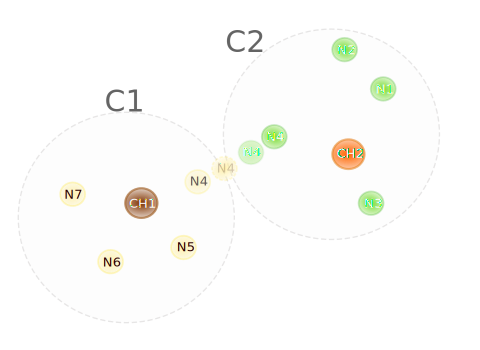
\includegraphics[scale=0.6, natwidth=0.38\textwidth]{scenario01}
  \end{center}
  \caption{Time line Showing the Cluster head communication}
\end{figure}

\begin{figure}[h]{} 
	\label{fig:timing}
  \begin{center}
    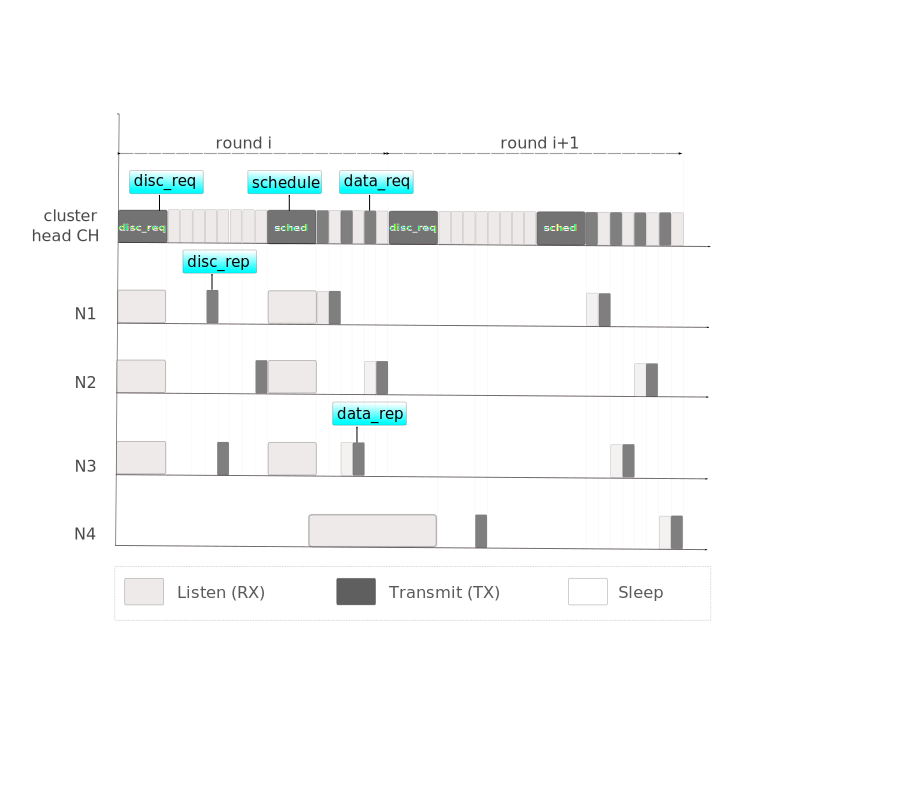
\includegraphics[scale=0.45, natwidth=0.38\textwidth]{timing-dia}
  \end{center}
  \caption{Time line Showing the Cluster head communication}
\end{figure}


To understand our approach, lets consider the scenario depicted in figure \ref{fig:scenario}. There are two clusters $C_1$ and $C_2$. Each cluster consists of a few mobile nodes and a cluster head (CH$_1$,CH$_2$). Notice that node \emph{$N_4$} moves from $C_1$ to $C_2$. When N4 moves out of the range of CH$_1$, it stops receiving the periodic data request message from CH$_1$. Realizing that it has moved out of cluster $C_1$, N4 switches its radio to listen mode, listening for \emph{disc\_req} packet from other cluster heads. After waiting a while, it receives a \emph{disc\_req} message from CH$_2$ as shown in figure \ref{fig:timing}. N4 chooses one of the slots in the discovery reply phase to send a \emph{disc\_rep} packet. CH$_2$ adds N4 to the schedule and broadcast the schedule. N4 acquires its data transfer slot timing from the schedule. During its slot, N4 wakes up to receive \emph{data\_req} packet from CH$_2$ and replies to it with a \emph{data\_rep} packet. Using the next data transfer session schedule acquired from the \emph{data\_req} packet, N4 sets a timer and puts its radio in sleep mode. 

%%%%%%%%%%%%%%%%%%%%%%%%%%%%%%%%%%%%%%%%%%%%%%%%%%%%%%%%%%%%%%%%%%
\iffalse 
In this section we will discuss the working of our protocol from a mobile node and from a static node's perspective. 

--- Try framing an algorithm w.r.t the static node. \\

Try framing an algorithm w.r.t the mobile node. \\

Try framing an algorithm w.r.t the timeslot allocation b/w the static node during the network initialization. \\ \\

Sample Algorithm
% ------------------------------------------------------- %
\alglanguage{pseudocode}
\begin{algorithm}[H]
\caption{D-TDMA MAC}
\begin{algorithmic}[1]
\Procedure {DTDMA\_MAC}{$P_c$, $N$, $R$, $a$, $\Re$}
    \State $T \leftarrow \frac{R}{a}$
      
\EndProcedure
\end{algorithmic}
\end{algorithm}
\fi
%%%%%%%%%%%%%%%%%%%%%%%%%%%%%%%%%%%%%%%%%%%%%%%%%%%%%%%%%%%%%%%%%%
\section{Simulation and Results}
\label{sim}
stuff thangs.. coraaaaaaal.. stuff thangs.. coraaaaaaal..
stuff thangs.. coraaaaaaal..  stuff thangs.. coraaaaaaal..

% ------------------------------------------------------- %
\subsection{Performance Evaluation}         

Results comes here
Comparison to be done with Hybrid MAC and Mobi Sense

%%%%%%%%%%%%%%%%%%%%%%%%%%%%%%
\section{Conclusion}
\label{conclusion}
This paper proposes a TDMA based MAC protocol for Mobile Wireless Sensor Networks. The primary goal of the approach is to increase the sleep time of mobile nodes, there by increasing their lifetime. The use of Data Request message improves the reliability of the data transfer and also informs the mobile node about its data transfer slot during the next round. Implementation of D-TDMA is done in Castalia Simulator. We have compared our results with that of \cite{hmac} and observed that our approach performs better in terms of scalability, throughput, packet delivery ratio and energy efficiency.

\bibliographystyle{ieeetr}
\bibliography{OPA}
\end{document}

